% !TeX spellcheck = es_ES
\chapter{Experimental}
\label{ch:chap05}

\section{Ambiente de prueba}
\label{sec:hardware}

\begin{table}[H]
	\centering
	\begin{tabular}{l|l}
		Procesador & Intel i7 8700K - 12 CPUs - 3.7 GHz       \\
		\hline
		GPU        & Nvidia GeForce GTX 1070 Ti - 8 GiB  VRAM \\
		\hline
		RAM        & 32 GiB - 2667 MHz                        \\
		\hline
	\end{tabular}
	\caption{Características del hardware utilizado}
\end{table}

\begin{table}[H]
	\centering
	\begin{tabular}{l|l}
	SO & Windows 10 Pro        \\
		\hline
	Embree        & v3.5.2 \\
		\hline
		OpenGL        & v4.5  \\
		\hline
	\end{tabular}
	\caption{Características del hardware utilizado}
\end{table}

\section{Escenas}
\label{sec:escenas}

Con el objetivo de obtener resultados comparables para los distintos algoritmos y configuraciones se plantea el uso de dos escenas particulares de prueba, con distintas variaciones en los materiales que componen cada una de ellas.


\begin{figure}[H]
	\centering
	\begin{subfigure}{0.45\textwidth}
		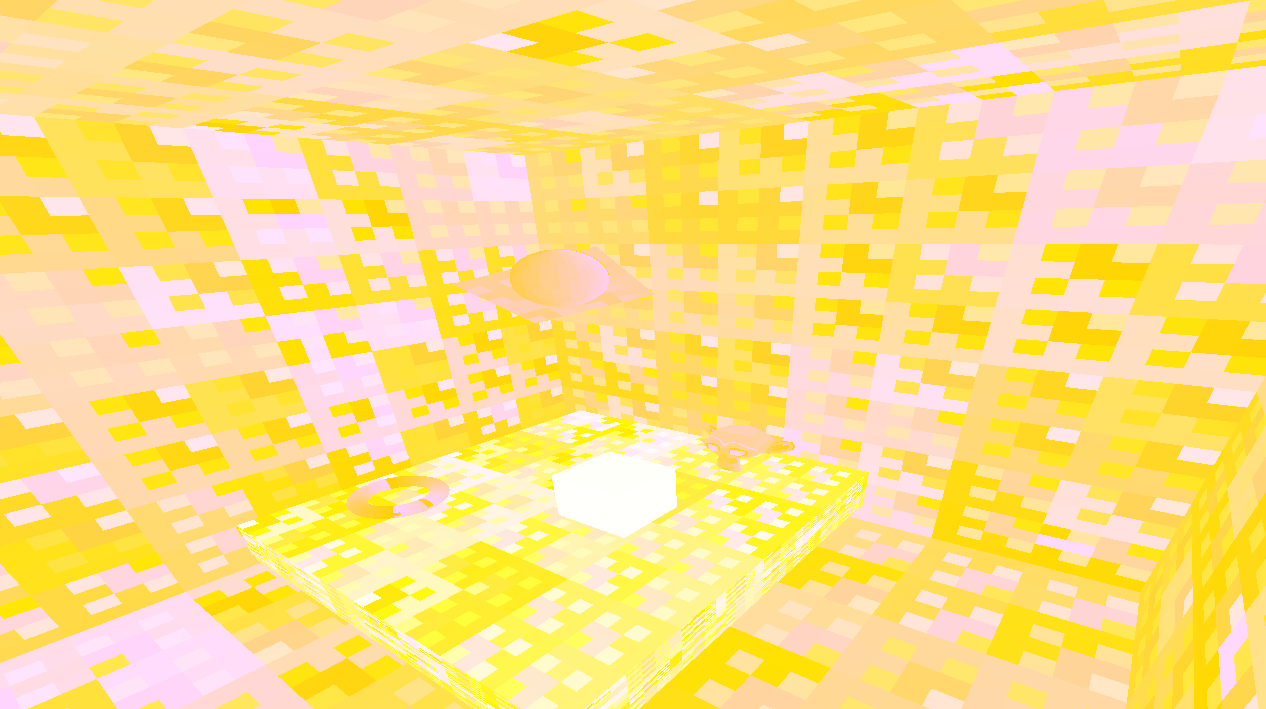
\includegraphics[width=1\linewidth]{assets/cornell}
		\caption{Vista lateral}
	\end{subfigure}
	\begin{subfigure}{0.45\textwidth}
		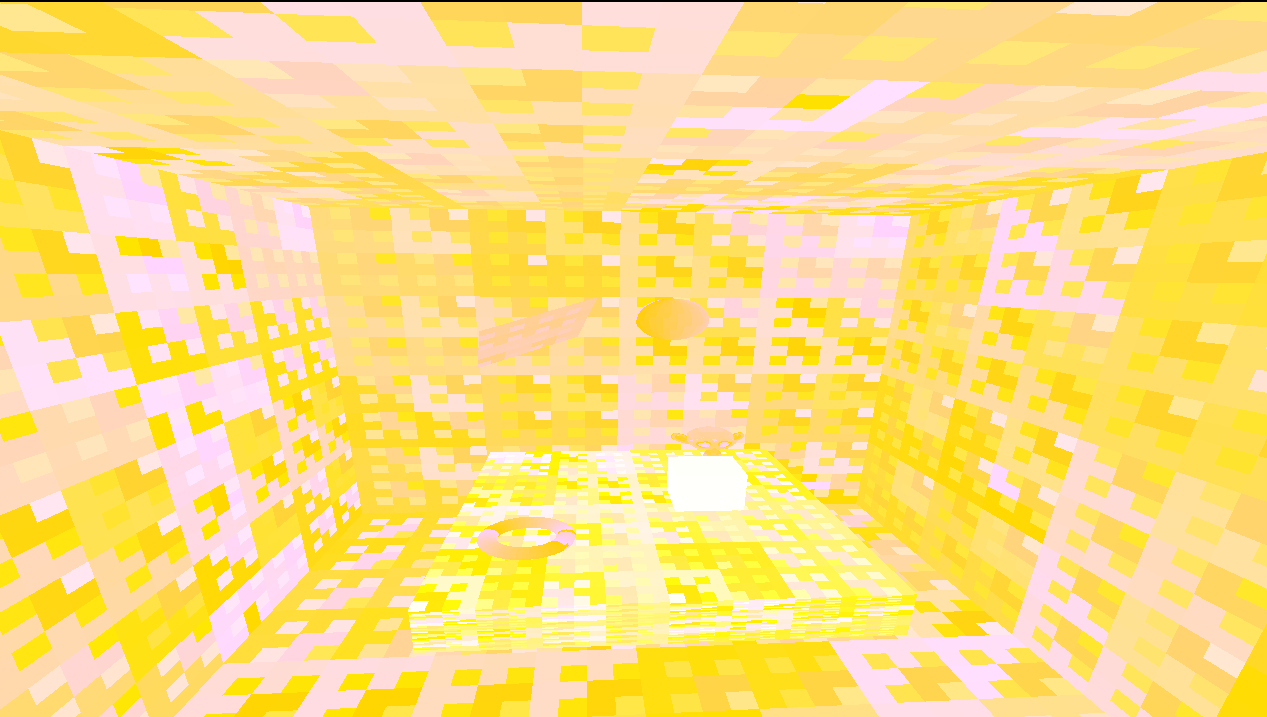
\includegraphics[width=1\linewidth]{assets/cornell2}
		\caption{Vista frontal}
	\end{subfigure}
	\caption{Vistas de la escena \textit{Conrnell Box}}
	\label{img:cornell}
\end{figure}

Se denominará \textit{Escena - Conrnell Box} a la referente a la figura \ref{img:cornell}. Se basa en un tipo de escena comúnmente usado en el se ubican objetos en el interior de una caja (cubo) donde debajo están los objetos de prueba y en el nivel superior reside el objeto que emitirá luz. Esta escena cuenta con siete objetos, el cubo, una esfera que oficia de luz, y cinco objetos compuestos por diversas primitivas. En total, existen 12.922 caras de las cuales 96 son triangulares y 12.826 son cuadrilaterales. Cabe notar, que de haber soportado únicamente caras triangulares se procesarían 25.748 parches.


\begin{figure}[H]
	\centering
	\begin{subfigure}{0.45\textwidth}
		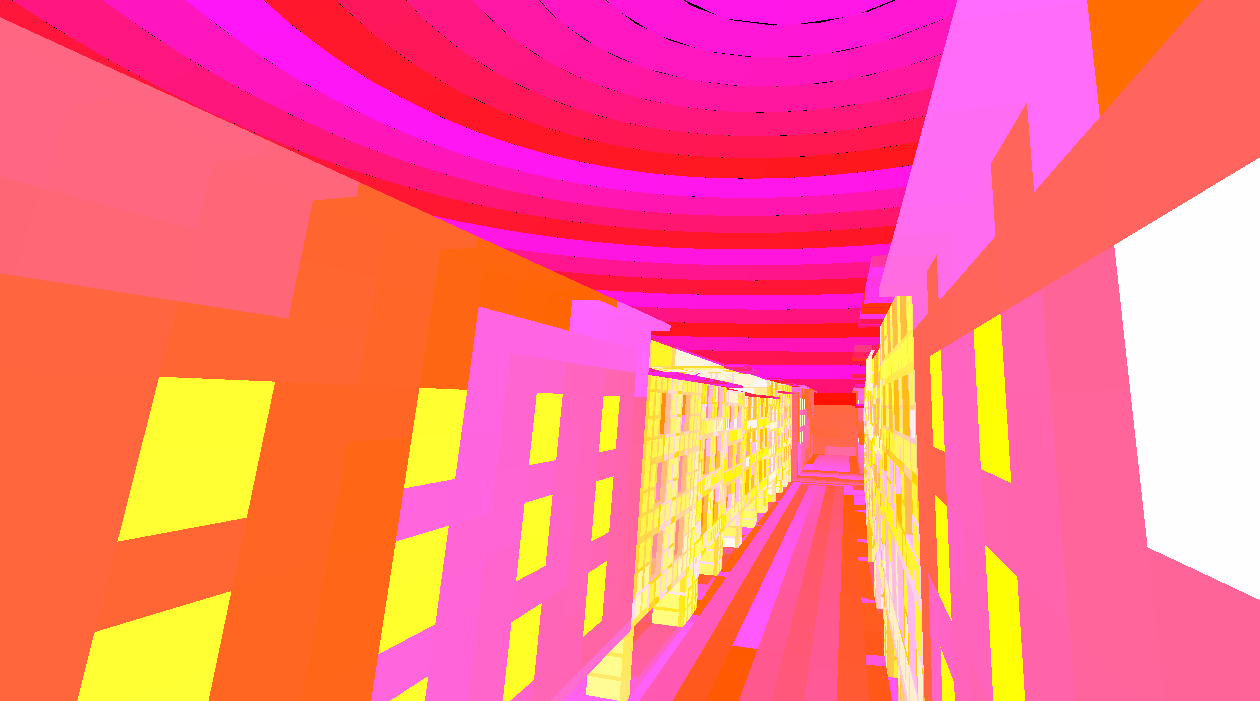
\includegraphics[width=1\linewidth]{assets/street1}
		\caption{Vista desde la ventana de una de las edificaciones}
	\end{subfigure}
	\begin{subfigure}{0.45\textwidth}
		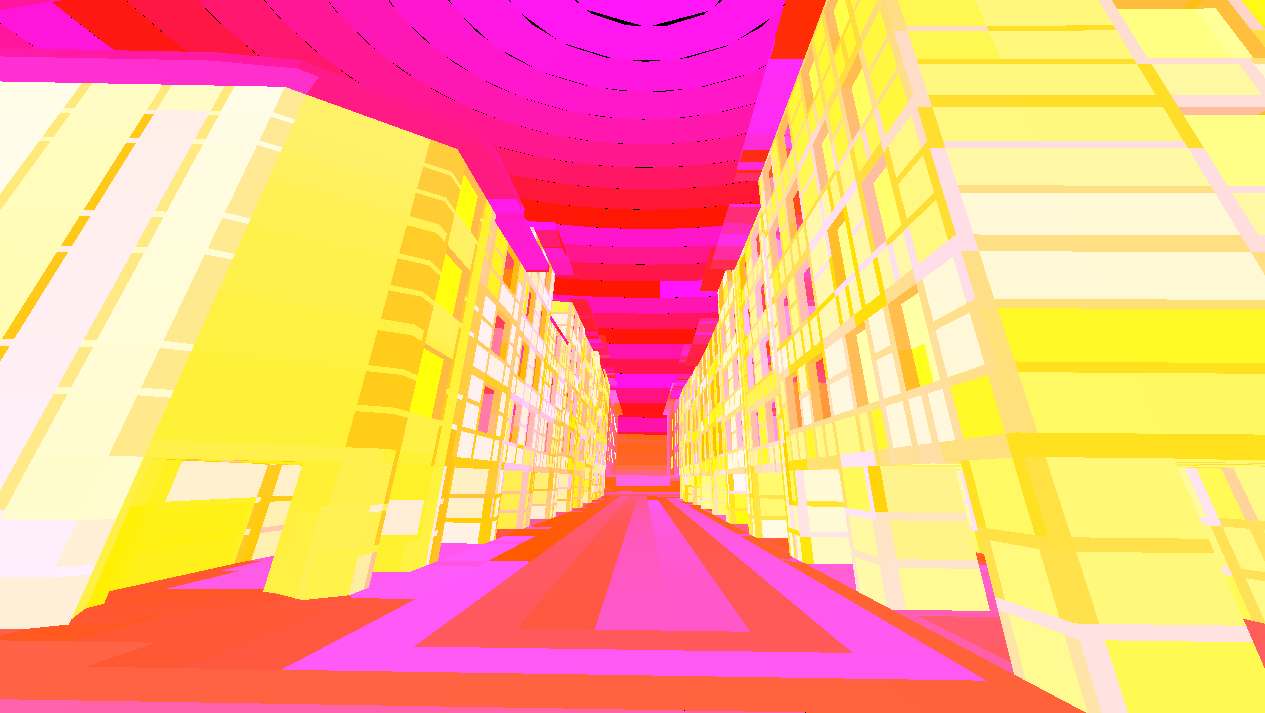
\includegraphics[width=1\linewidth]{assets/street2}
		\caption{Vista desde uno de los extremos de la calle}
	\end{subfigure}
	\begin{subfigure}{0.45\textwidth}
		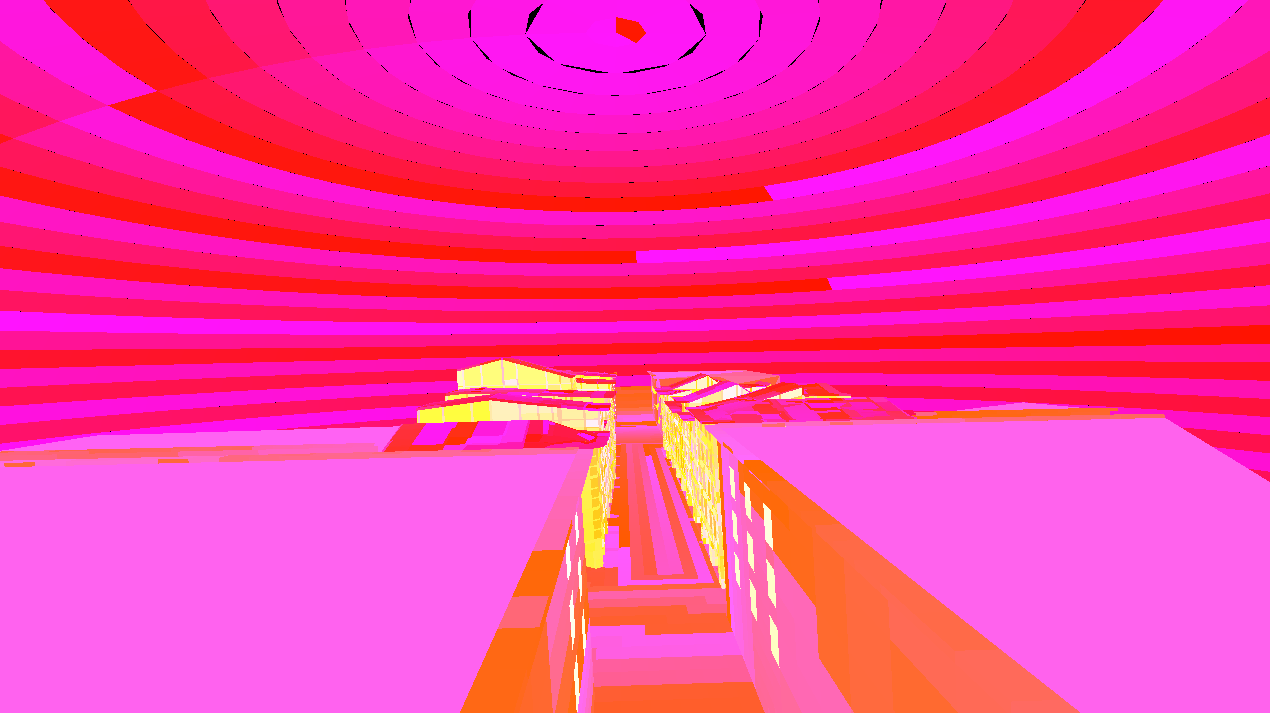
\includegraphics[width=1\linewidth]{assets/street3}
		\caption{Vista aérea}
	\end{subfigure}
	\begin{subfigure}{0.45\textwidth}
		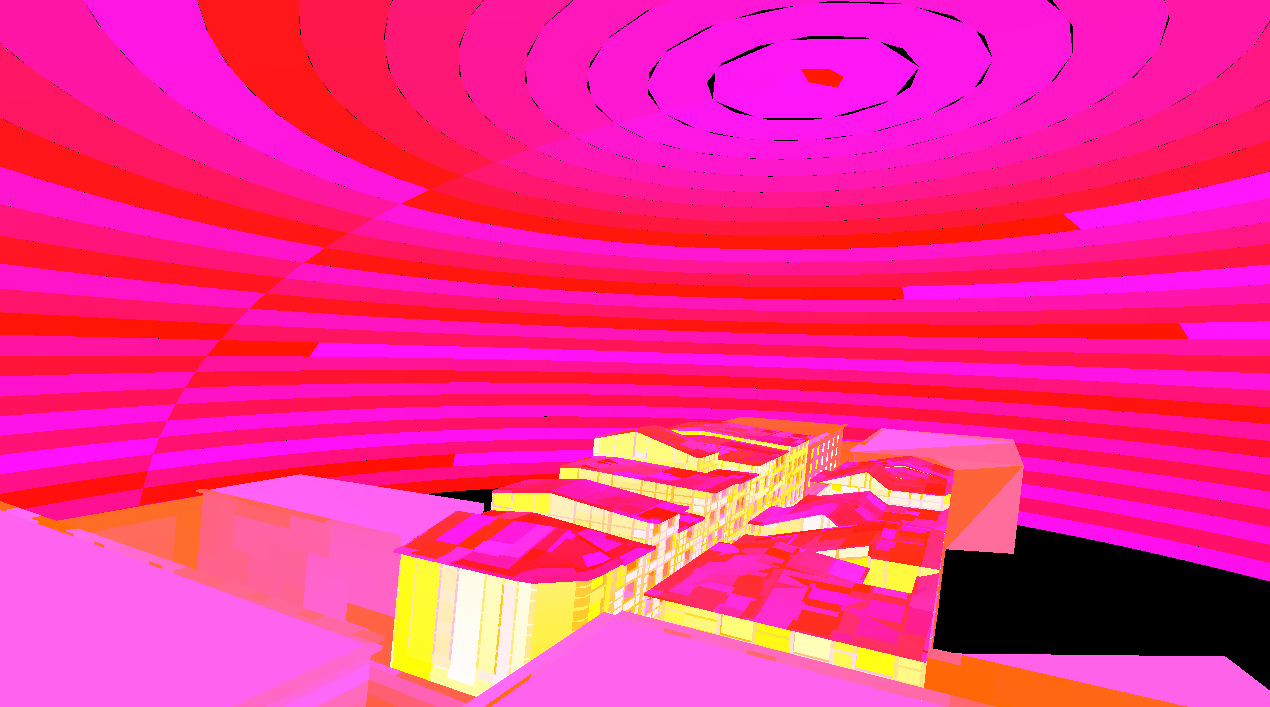
\includegraphics[width=1\linewidth]{assets/street4}
		\caption{Vista aérea}
	\end{subfigure}
	\caption{Vistas de la escena \textit{Calle}}
	\label{img:street}
\end{figure}

Se denominará \textit{Escena - Calle} a la referente a la figura \ref{img:street}. La escena está construida por dos objetos, el primero de ellos es una cúpula (hemi-esfera) subdividia en 2.407 cuadriláteros de área equitativa, su objetivo es representar el cielo. Por otro lado, el segundo objeto es una representación de una porción de una calle en el barrio de Petit Bayonne, localizado en Bayona, Francia cuyas imágenes se aprecian en la figura \ref{img:streetcomp}. El modelo fue construido por \citeauthor{Benoit} con el objetivo de estudiar el fenómeno de la radiación. En total, las escena cuenta con 61.795 caras cuadrilaterales.


\begin{figure}[H]
	\centering
	\begin{subfigure}{0.475\textwidth}
		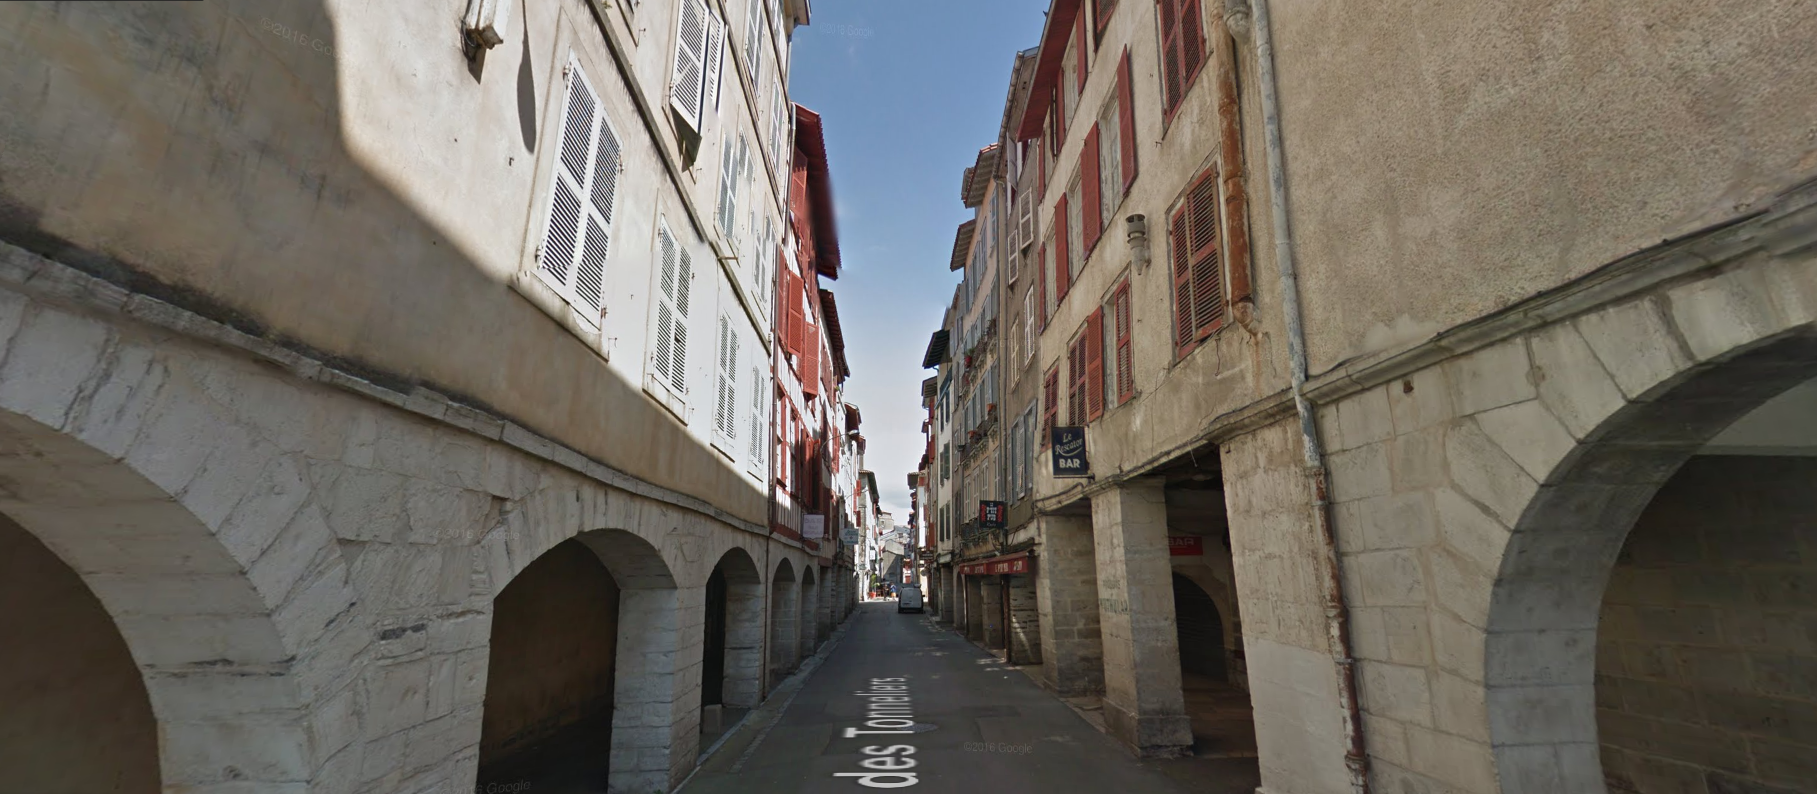
\includegraphics[width=1\linewidth]{assets/streetreal1}
		\caption{Vista Sur - real}
	\end{subfigure}
	\begin{subfigure}{0.475\textwidth}
		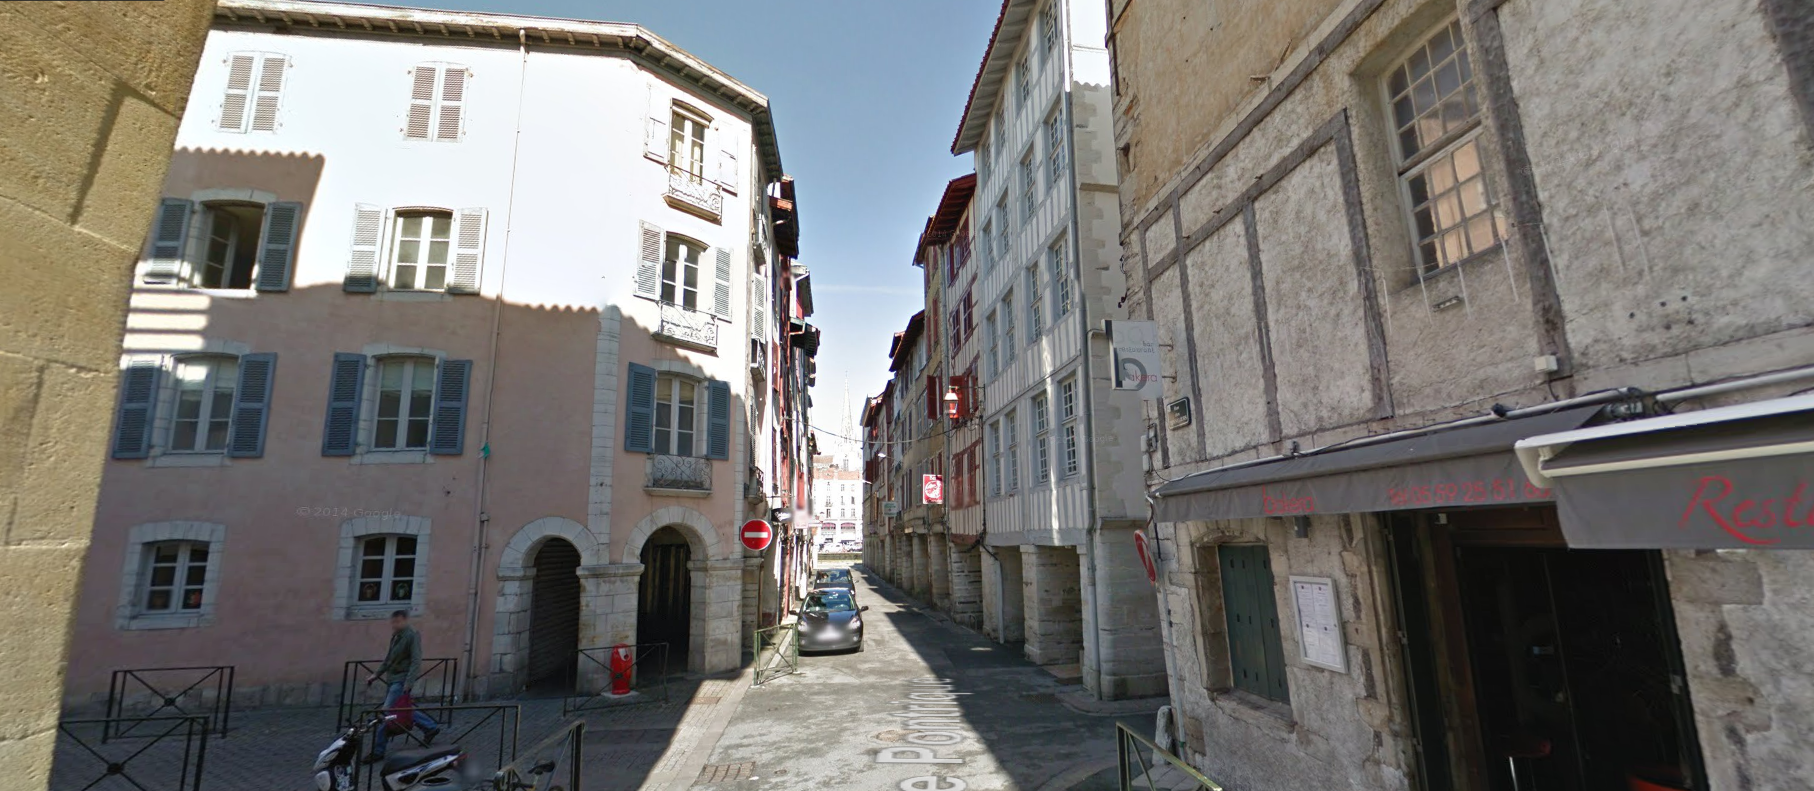
\includegraphics[width=1\linewidth]{assets/streetreal2}
		\caption{Vista Norte - real}
	\end{subfigure}
	\begin{subfigure}{0.475\textwidth}
		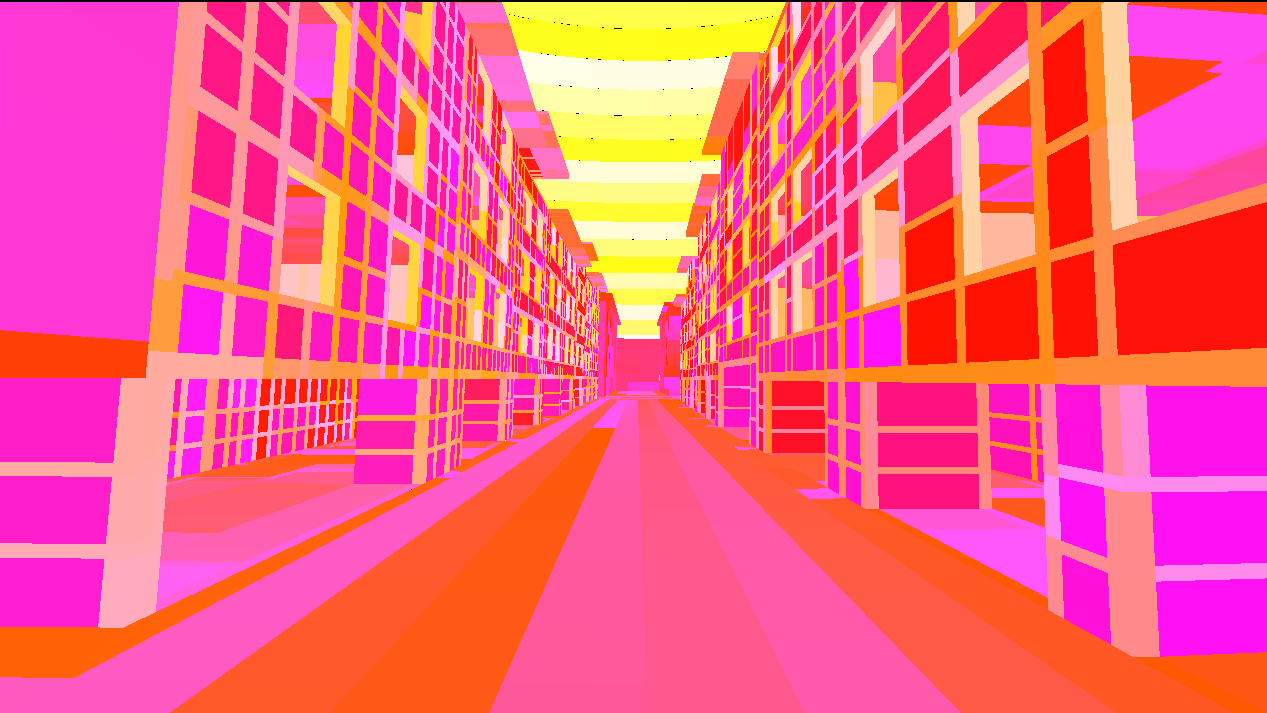
\includegraphics[width=1\linewidth]{assets/streetmodel1}
		\caption{Vista Sur - modelada}
	\end{subfigure}
	\begin{subfigure}{0.475\textwidth}
		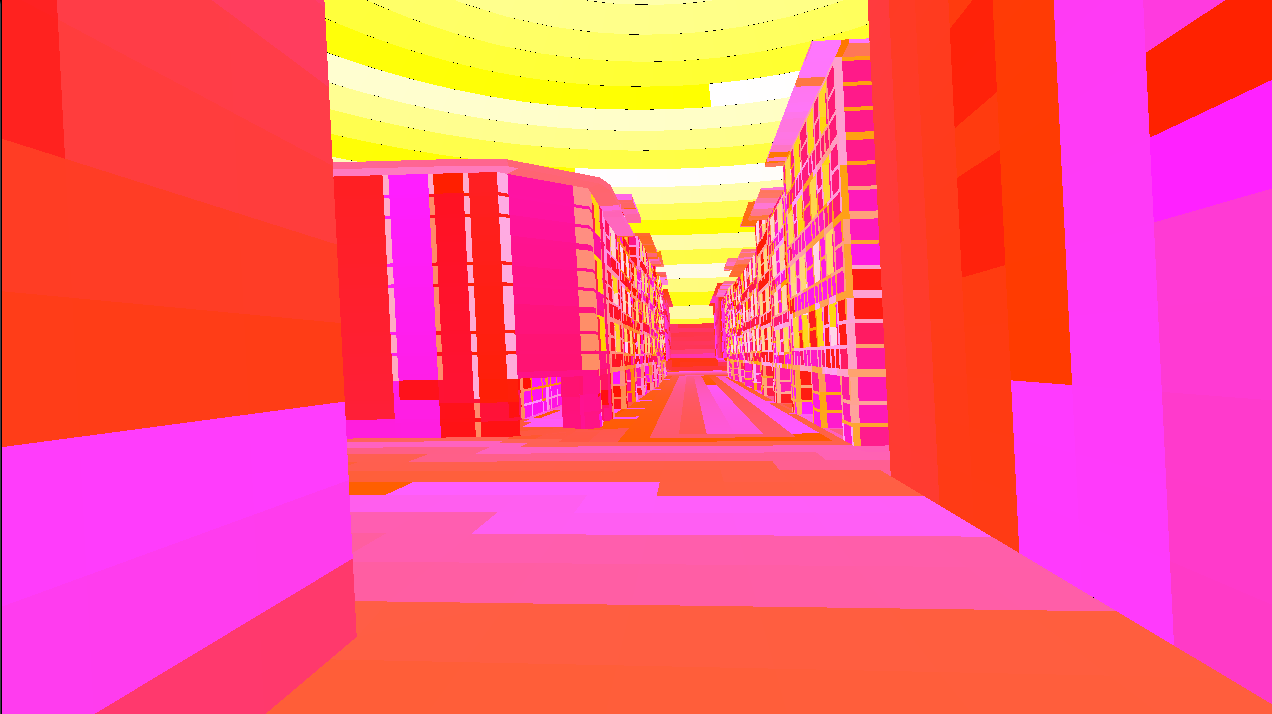
\includegraphics[width=1\linewidth]{assets/streetmodel2}
		\caption{Vista Norte - modelada}
	\end{subfigure}
	\caption{Comparación entre el fotografías reales del modelo \textit{Calle} y su representación tridimensional}
	\label{img:streetcomp}
\end{figure}

\section{Casos de prueba}
\label{sec:pruebas}

Se proponen casos de prueba utilizando las escenas descritas en \ref{sec:escenas} utilizando diversos materiales.

\subsection{Métricas consideradas}
\label{metricasestablecidas}
Con el objetivo de medir correctamente las ventajas y desventajas de cara acercamiento al cálculo de factores de forma simples y extendidos que se han propuesto, se definirán un conjunto de métricas para evaluar su optimialidad en distintas dimensiones. Cada dimensión considerada se aplicará dependiendo del caso considerado.

\begin{itemize}
	\item Dimensión rendimiento
		\begin{itemize}
			\item Tiempo de ejecución: Se registrará el tiempo empleado en calcular completamente la matriz de factores de forma.
		\end{itemize}
	\item Dimensión matriz de factores de forma: Se computará la matriz de factores de forma de control $\mathbf{F_{C}}$ utilizando la técnica de trazado de rayos con una gran resolución.
		\begin{itemize}
			\item Error promedio de factor de forma por fila: $Ep_{i} = \sum_{j=1}^{N} \frac{|\mathbf{F_{C}}_{ij} -\mathbf{F}_{ij}|}{N}$
			\item Error máximo de factor de forma por fila: $Em_{i} = \max_{j=1}^{N}|\mathbf{F}_{ij} -\mathbf{Fc}_{ij}|$
			\item Error estándar de factor de forma por fila: $Em_{i} = \max_{j=1}^{N}(\mathbf{F}_{ij} -\mathbf{F_{C}}_{ij})^{2}$
		\end{itemize}
	\item Dimensión vector de radiosidad (dado el vector $R$, y el vector de control $Rc$):
	\begin{itemize}
		\item Error promedio de radiosidad: $Ep = \sum_{i=1}^{N} \frac{|R_{i}-R_{Ci}|}{N}$
		\item Error máximo de radiosidad: $Em = \max_{j=1}^{N}|R_{j} -Rc_{j}|$
		\item Error estándar de radiosidad: $Em = \max_{j=1}^{N}(R_{j} -Rc_{j})^{2}$
	\end{itemize}
\item Dimensión visual:
	\begin{itemize}
		\item Calidad de resultados: Se evaluarán los resultados esperando que se asemejen a la realidad.
	\end{itemize}
\end{itemize}

\subsection{Descripción de casos de prueba}

\begin{enumerate}
	\item \textit{Pruba difusa}: Se utilizarán materiales estrictamente difusos en ambas escenas, con colores aleatorios. Desactivando, entonces, cualquier interacción especular. Se escogerá un conjunto de parches que oficiarán de fuente luminosa. En caso de la escena \textit{Calle}, se seleccionan 10 parches que emulan la luz solar. Por otro lado, para la escena \textit{Cornell Box} se utiliza la bola central como fuente luminosa.
	\item \textit{Pruba especular}: Se utilizarán materiales difusos y especulares en ambas escenas, con una cantidad reducida de estos últimos. En caso de la escena \textit{Cornell Box} se utiliza el plano ubicado en el centro como reflector, mientras que en la escena \textit{Calle} se utiliza una selección de ventanas. Para cada \textit{pipeline} (completo) implementado se computa la radiosidad registrando el tiempo de renderizado según la cantidad de muestras configurada.
	\item \textit{Prueba híbrida}: Únicamente en la escena \textit{Cornell Box} se computarán dos variantes. En una de ellas se desactivan los reflectores especulares (plano) y en el otro caso no.
	\item{Prueba de estrés}: Se utiliza gran cantidad de espejos en ambas escenas.
\end{enumerate}

\subsection{Resultados observados}

\subsubsection{Caso de prueba I}

\begin{table}[H]
	\label{tab:tablecaso1}
	\centering
	\begin{tabular}{|c|l|l|l|l|}
		\hline
		\multirow{3}{*}{\textbf{Muestras}} & \multicolumn{4}{c|}{\textbf{Tiempo de ejecución (s)}}                                                                                  \\ \cline{2-5} 
		& \multicolumn{2}{c|}{\textit{Cornell Box}}                 & \multicolumn{2}{c|}{\textit{Calle}}                      \\ \cline{2-5} 
		& \multicolumn{1}{c|}{OpenGL} & \multicolumn{1}{c|}{Embree} & \multicolumn{1}{c|}{OpenGL} & \multicolumn{1}{c|}{Embree} \\ \hline
		\textbf{96}                        & 7                           & 3                           & 68                          & 14                          \\ \hline
		\textbf{384}                       & 10                          & 30                          & 128                         & 174                         \\ \hline
		\textbf{768}                       & 31                          & 116                         & 248                         & 665                         \\ \hline
		\textbf{1536}                      & 251                         & 446                         & 1213                        & 2565                        \\ \hline
		\textbf{3072}                      & 992                         & 1778                        & 4018                        & 7511                        \\ \hline
	\end{tabular}
	\caption{Resultados obtenidos para el primer caso de prueba en ambas escenas consideradas}
\end{table}

En este caso, se observa en la tabla \ref{tab:tablecaso1} que el método del hemicubo tiene un rendimiento considerablemente superior al de la traza de rayos. Cabe destacar que se observó una ocupación promedio de la GPU del 30\% y CPU 90\% (esta última probablemente se deba a la gran cantidad de sincronizaciones necesarioas entre el dispositivo y el controlador); mientras que el uso de traza de rayos presentó una ocupación de los núcleos del procesador del 99\%. Se destaca la diferencia observada entre OpenGL y Embree en \ref{plot:emglc1}.

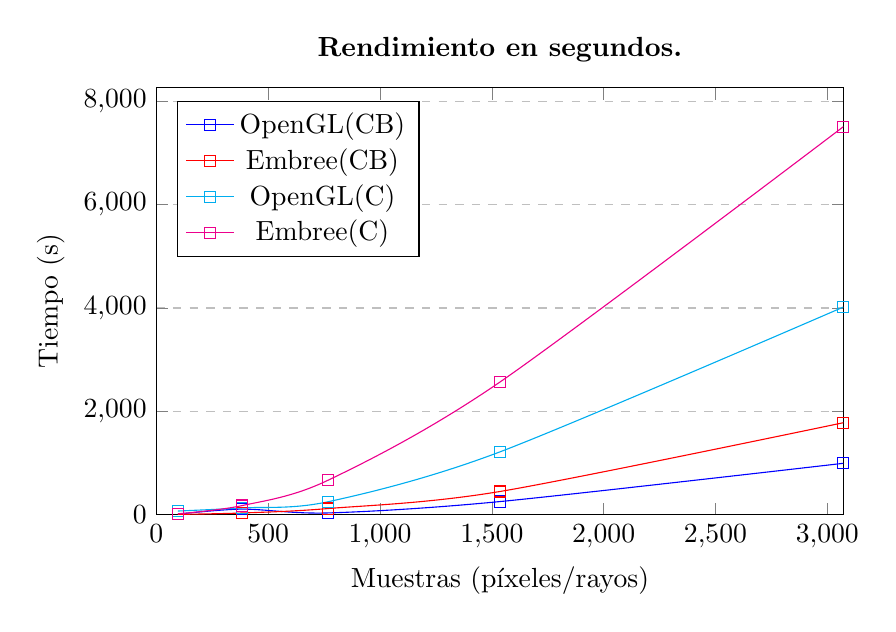
\begin{tikzpicture}
\label{plot:emglc1}
\begin{axis}[
title={\textbf{Rendimiento en segundos.}},
xlabel={Muestras (píxeles/rayos)},
ylabel={Tiempo (s)},
xmin=0, xmax=3072,
ymin=0,
width=.85\textwidth, height=7cm,
legend pos=north west,
ymajorgrids=true,
grid style=dashed,
]

\addplot[
smooth,
color=blue,
mark=square,
]
coordinates {
	(96,7)(384,105)(768,31)(1536,251)(3072,992)
};
\addplot[
smooth,
color=red,
mark=square,
]
coordinates {
	(96,3)(384,30)(768,116)(1536,446)(3072,1778)
};

\addplot[
smooth,
color=cyan,
mark=square,
]
coordinates {
	(96,68)(384,128)(768,248)(1536,1213)(3072,4018)
};

\addplot[
smooth,
color=magenta,
mark=square,
]
coordinates {
	(96,14)(384,174)(768,665)(1536,2565)(3072,7511)
};

\legend{OpenGL(CB),Embree(CB),OpenGL(C), Embree(C)}

\end{axis}
\end{tikzpicture}

Una de las consecuencias más interesantes a ser analizadas para detectar la cantidad de muestras óptimas a considerar es la calidad de la imagen final, y qué tan pronunciados son las diferencias en de iluminación entre los parches, es decir, en qué medida difiere la radiosidad entre parches. Para este caso, se pudo observar (véase la figura \ref{img:difres}) que si bien las resoluciones más bajas consumen menor cantidad de recursos los resultados tienen una calidad sustancialmente menor a la esperada. Considerando que el modelo generalmente es utilizado para el cálculo de mapas de iluminación en una etapa de pre-procesado, es recomendable evitar el uso de factores de muestreo tan bajos. Esto se ve acentuado en el análisis de la matriz de factores de forma, según las métricas establecidas en \ref{metricasestablecidas} se pudo comprobar que máximo error promedio apreciado (medida que se ha denominado $Ep$) fue de $4.15 10^{-5}$ y $3.91 10^{-5}$ utilizando $1536$ muestras para los métodos del hemicubo y la hemiesfera mientras que el uso de $96$ muestras generó errores del entorno de los $3.10 10^{-3}$ y $8.52 10^{-4}$ respectivamente. Estos errores se ven aún más acentuados al realizar el calcular la radiosidad para cada parche.

\begin{figure}[H]
	\centering
	\begin{subfigure}{0.45\textwidth}
		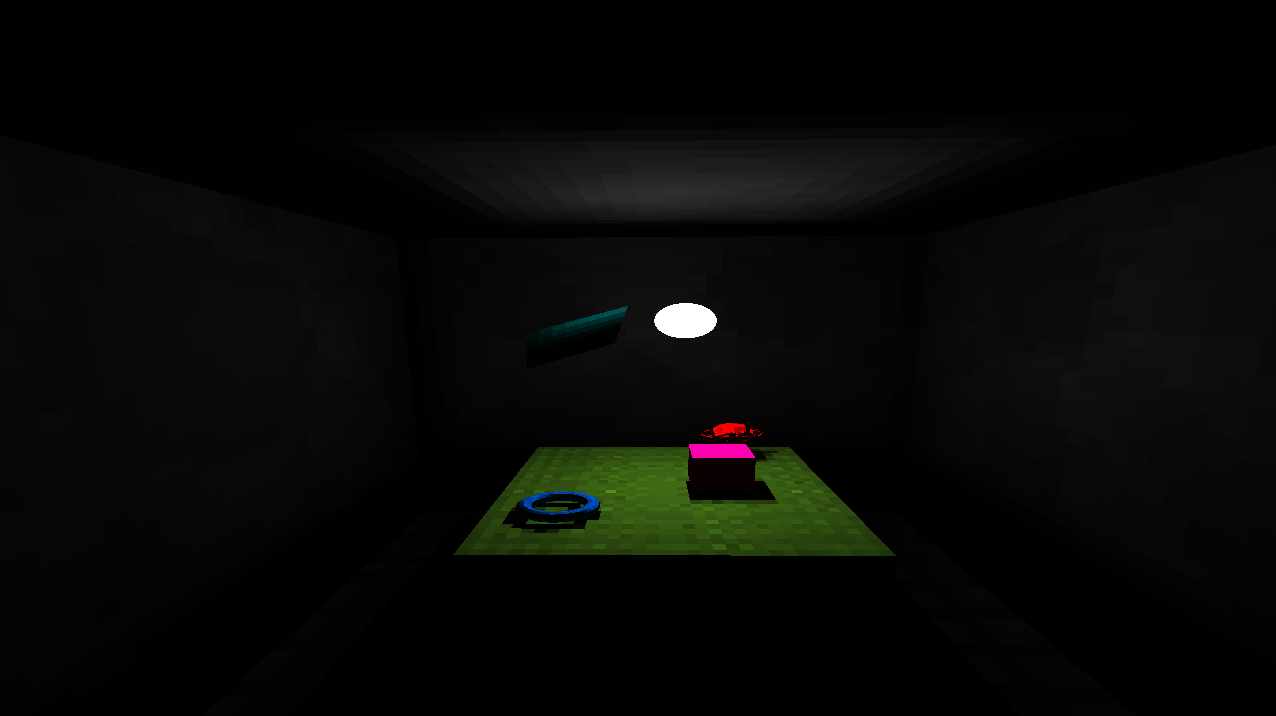
\includegraphics[width=1\linewidth]{assets/32sgl}
		\caption{OpenGL - 32 píxeles por cara}
	\end{subfigure}
	\begin{subfigure}{0.45\textwidth}
		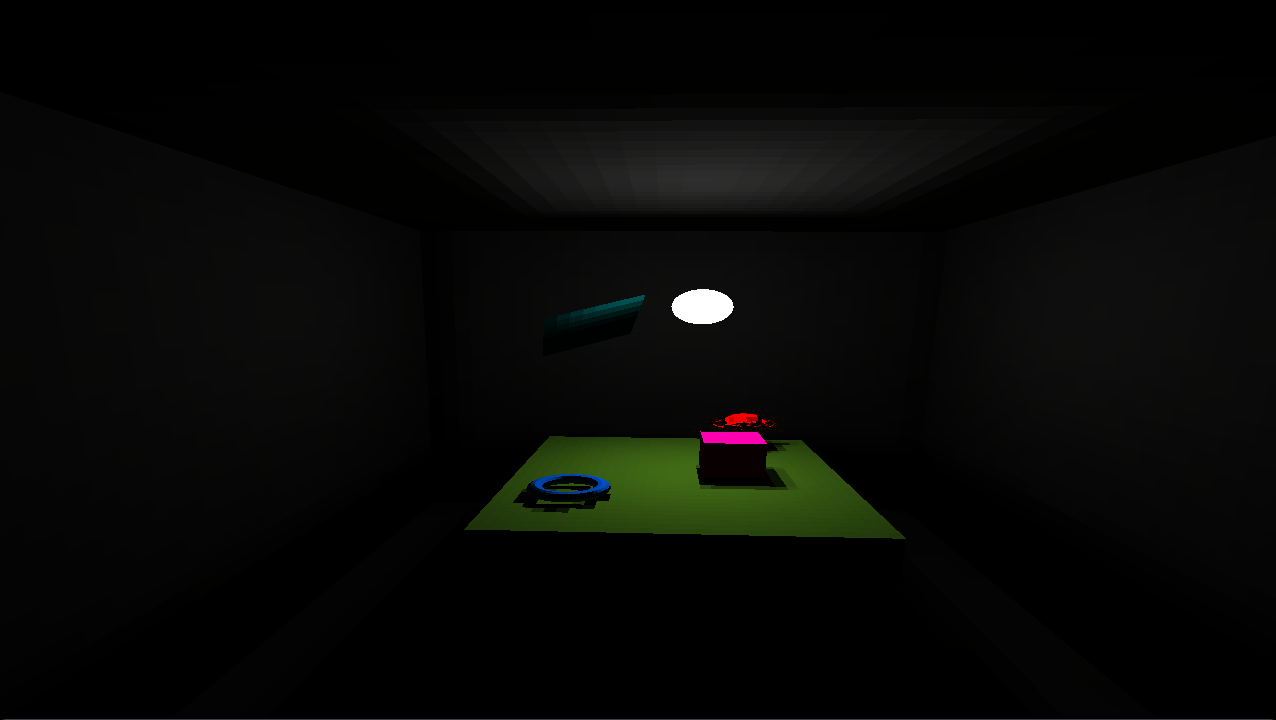
\includegraphics[width=1\linewidth]{assets/512sgl}
		\caption{OpenGL - 512 píxeles por cara}
	\end{subfigure}
	\begin{subfigure}{0.45\textwidth}
		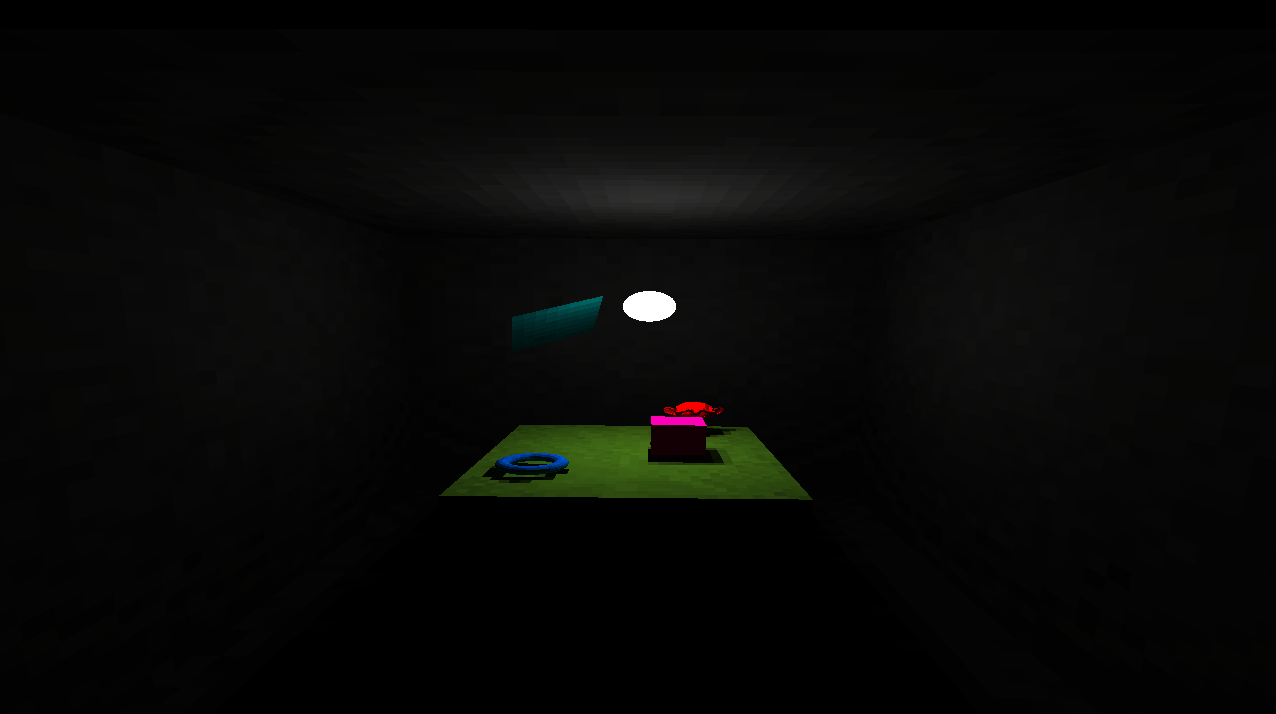
\includegraphics[width=1\linewidth]{assets/32srt}
		\caption{Embree - 96 rayos}
	\end{subfigure}
	\begin{subfigure}{0.45\textwidth}
		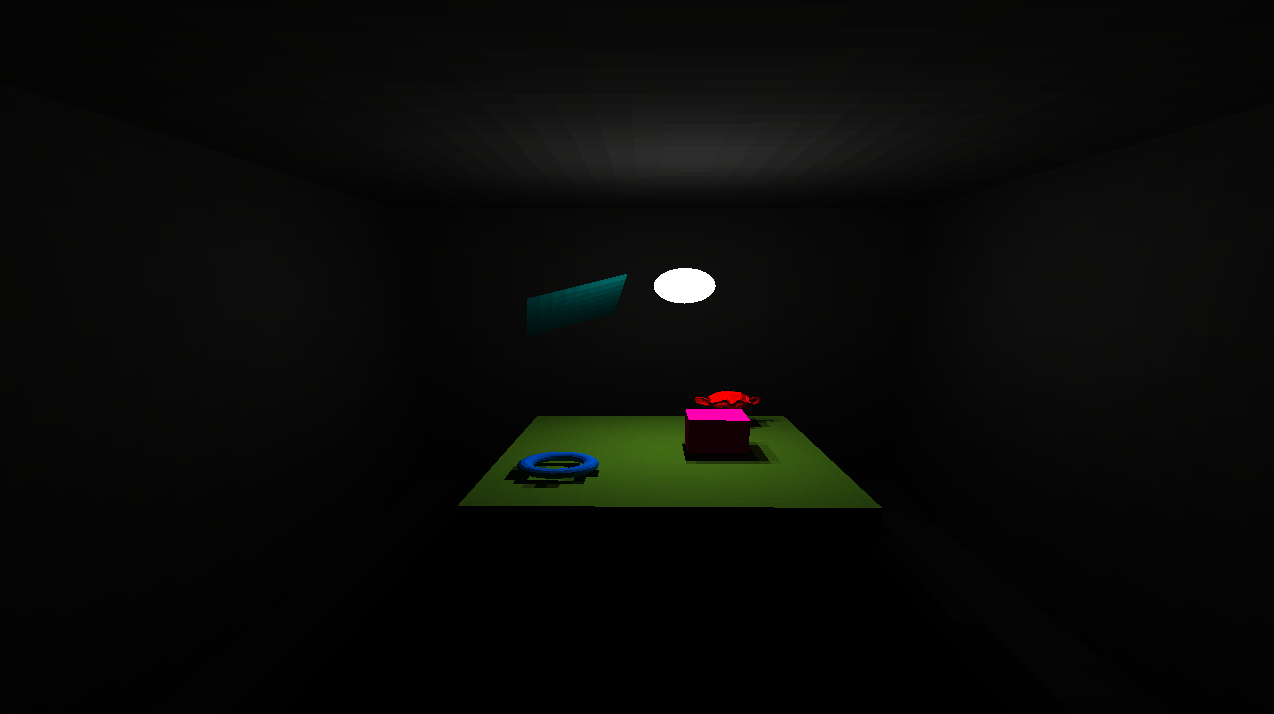
\includegraphics[width=1\linewidth]{assets/512srt}
		\caption{Embree - 1536 rayos}
	\end{subfigure}
	\caption{Diferencias visuales ajustando la cantidad de muestras}
	\label{img:difres}
\end{figure}

\subsubsection{Caso de prueba II}

En este caso, en cuanto a rendimiento, se observa en la tabla \ref{tab:caso2} que el mejor rendimiento observado se obtiene utilizando el método híbrido, esto se debe a los hilos que ejecutan los cálculos correspondientes al rebote especular (utilizando traza de rayos) son ejecutados en la CPU mientras la GPU procesa hemicubos. Esto se ve respaldado por el hecho de que, en promedio se observó una ocupación rondando en los entornos de 100\% de la CPU y 35\% GPU en el método híbrido; 75\% de la CPU y 30\% GPU en el método utilizando OpenGL y 99\% en la implementación que solo utiliza traza de rayos. 


\begin{table}[H]
	\centering
	\label{tab:caso2}
	\caption{Resultados obtenidos en el segundo caso de prueba}
	\begin{tabular}{|l|l|l|l|l|l|l|}
		\hline
		\multicolumn{1}{|c|}{\multirow{3}{*}{Muestras}} & \multicolumn{6}{c|}{Tiempo de ejecución (s)}                                                                                         \\ \cline{2-7} 
		\multicolumn{1}{|c|}{}                          & \multicolumn{3}{c|}{\textit{Cornell Box}}                                                & \multicolumn{3}{c|}{\textit{Calle}}      \\ \cline{2-7} 
		\multicolumn{1}{|c|}{}                          & \multicolumn{1}{c|}{OpenGL} & \multicolumn{1}{c|}{Embree} & \multicolumn{1}{c|}{Híbrido} & OpenGL                 & Embree & Híbrido \\ \hline
		\textbf{96 - 32}                                & 152                         & 53                          & 21                           & 2563                   & 1221   & 943     \\ \hline
		\textbf{768 - 32}                               & 312                         & 134                         & 84                          & 4521                   & 2512   & 1643    \\ \hline
		\textbf{1536 - 64}                              & 1071                        & 486                         & 228                          & \multicolumn{1}{c|}{-} & 5342   & 4725    \\ \hline
	\end{tabular}
\end{table}

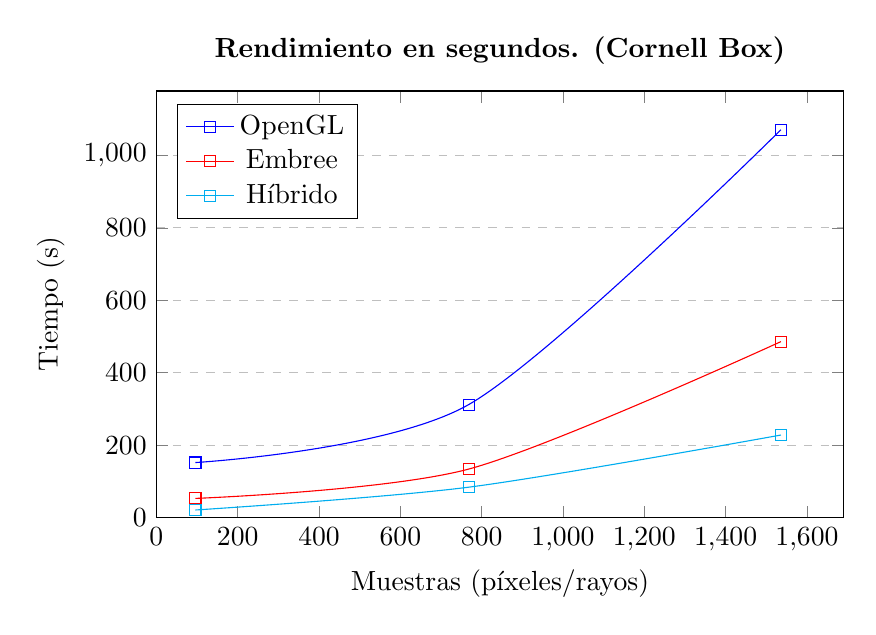
\begin{tikzpicture}
\label{plot:emglc2}
\begin{axis}[
title={\textbf{Rendimiento en segundos. (Cornell Box)}},
xlabel={Muestras (píxeles/rayos)},
ylabel={Tiempo (s)},
xmin=0,
ymin=0,
width=.85\textwidth, height=7cm,
legend pos=north west,
ymajorgrids=true,
grid style=dashed,
]

\addplot[
smooth,
color=blue,
mark=square,
]
coordinates {
	(96,152)(768,312)(1536,1071)
};
\addplot[
smooth,
color=red,
mark=square,
]
coordinates {
	(96,53)(768,134)(1536,486)
};

\addplot[
smooth,
color=cyan,
mark=square,
]
coordinates {
	(96,21)(768,84)(1536,228)
};


\legend{OpenGL,Embree,Híbrido}

\end{axis}
\end{tikzpicture}

El paralelismo de las implementaciones basadas en la GPU garantiza el mejor rendimiento, sin embargo, se pudo notar que el uso exclusivo de traza de rayos provee hasta 14 veces menor error máximo que los otros algoritmos implementados (en \textit{Cornell Box}, con 1536 muestras se notó una diferencia de error máxima $Ep$ de $6.78 10^{-5}$ con el método híbrido y  $9.13 10^{-4}$ utilizando el método de dibujado de portales). Esto se debe a que tanto en el uso de dibujado de portales o el algoritmo híbrido se utilizan estimaciones de la dirección en la que rebotaría el rayo en el espejo considerado, lo que degrada la autenticidad final de los datos obtenidos, sobre todo en el dibujado de portales donde la granularidad de las muestras obtenidas es inferior (se toman muestras por área y no por rayo). Por lo tanto, incluso si el método de traza de rayos posee un rendimiento un tanto menor (que se debe mayormente al hecho de que se ejecuta únicamente en la CPU) se observa una calidad de datos órdenes de magnitud superior a la de los otros métodos.

\begin{figure}[H]
	\centering
	\begin{subfigure}{0.5\textwidth}
		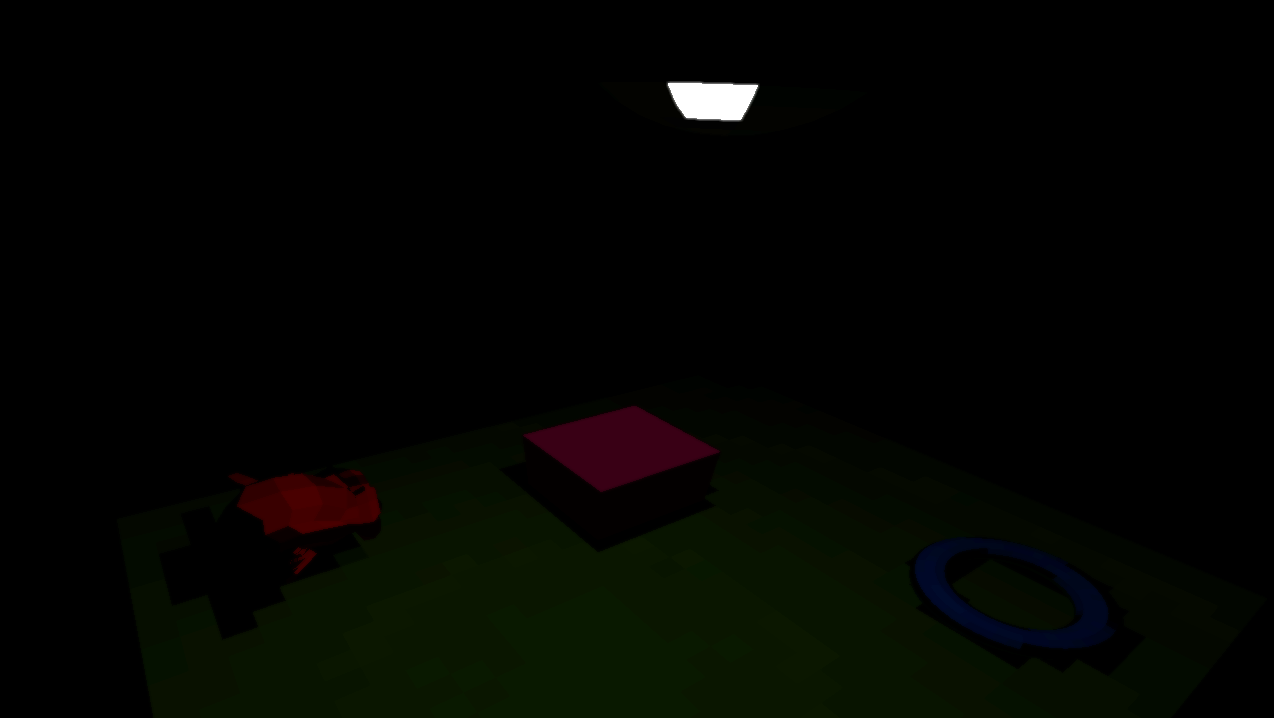
\includegraphics[width=1\linewidth]{assets/caso2gl}
		\caption{OpenGL}
	\end{subfigure}
	\begin{subfigure}{0.5\textwidth}
		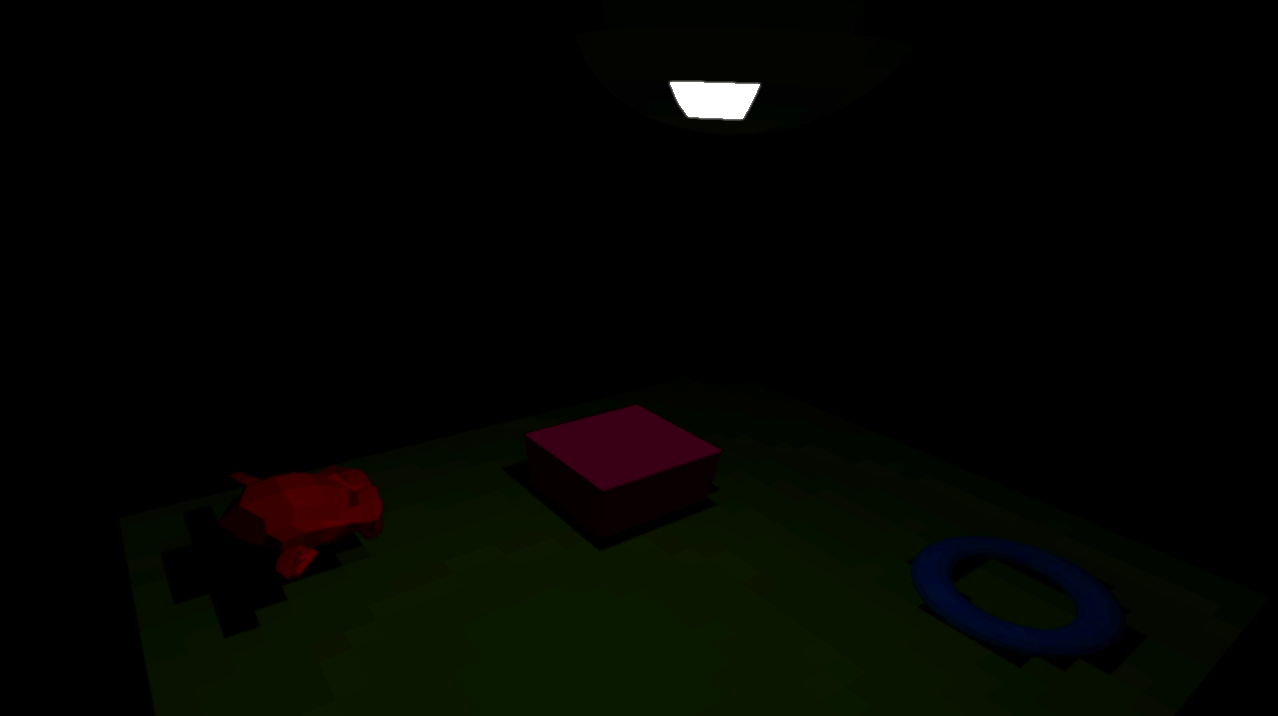
\includegraphics[width=1\linewidth]{assets/caso2e}
		\caption{Embree}
	\end{subfigure}
	\begin{subfigure}{0.5\textwidth}
		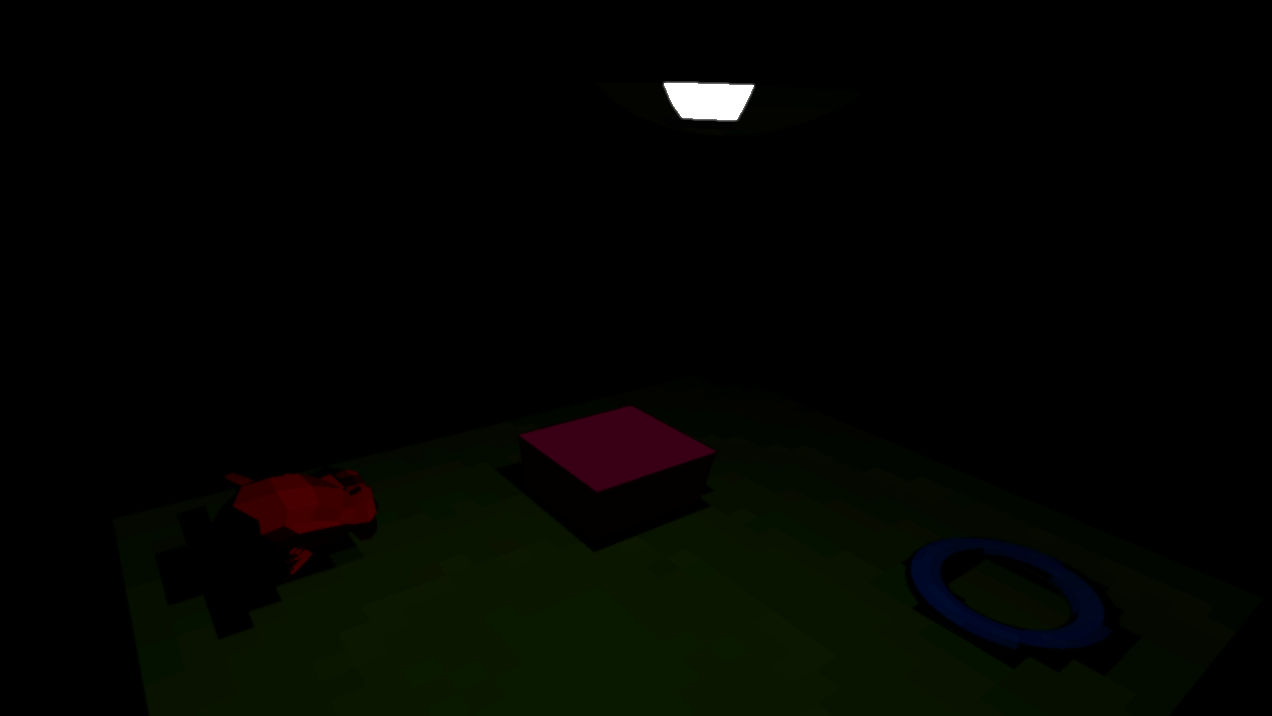
\includegraphics[width=1\linewidth]{assets/caso2h}
		\caption{Híbrido}
	\end{subfigure}	
	\caption{Diferencias visuales visualizadas utilizando las distintas implementaciones de factores de forma extendido. 1536 muestras iniciales y 64 para rebotes especulares.}
	\label{img:difres}
\end{figure}

Con el objetivo de cuantificar los datos de error observado se analizó el error estándar y promedio observado en el vector de radiosidad final (comparado a una muestra utilizando exclusivamente trazado de rayos con 3276 muestras para la hemiesfera) y se observó que, tal como se había supuesto, el método es significativamente menos propenso a generar errores como se ve en la figura \ref{plot:emglc1}.

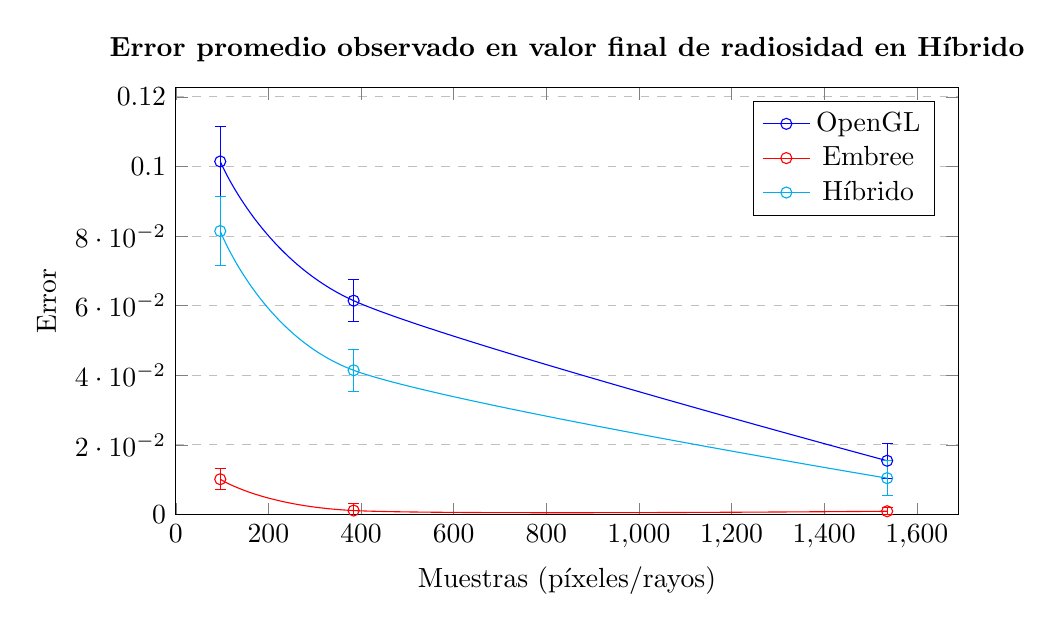
\begin{tikzpicture}
\label{plot:errorcII}
\begin{axis}[
title={\textbf{Error promedio observado en valor final de radiosidad en Híbrido}},
xlabel={Muestras (píxeles/rayos)},
ylabel={Error},
xmin=0,
ymin=0,
width=.95\textwidth, height=7cm,
legend pos=north east,
ymajorgrids=true,
grid style=dashed,
]

\addplot[
smooth,
color=blue,
mark=square,
mark=o,error bars/.cd, y dir=both,y explicit
]
coordinates {
	(96,0.10145) +- (0, 0.01)
	(384,0.06145) +- (0, 0.006)
	(1536,0.01545) +- (0, 0.005)
};
\addplot[
smooth,
color=red,
mark=square,
mark=o,error bars/.cd, y dir=both,y explicit
]
coordinates {
	(96,0.010145) +- (0, 0.003)
	(384,0.001145) +- (0, 0.002)
	(1536,0.000945) +- (0, 0.001)
};

\addplot[
smooth,
color=cyan,
mark=square,
mark=o,error bars/.cd, y dir=both,y explicit
]
coordinates {
	(96,0.08145)  +- (0, 0.01)
	(384,0.04145)  +- (0, 0.006)
	(1536,0.01045)  +- (0, 0.005)
};


\legend{OpenGL,Embree,Híbrido}

\end{axis}
\end{tikzpicture}

\subsubsection{Caso de prueba III}

Esta prueba se construyó con el objetivo de comparar el rendimiento observado utilizando los algoritmos de extensión de factores de forma implementados por lo que su análisis es escueto. Las pruebas se realizaron con una cantidad de muestras fijar (768 muestras de hemicubo/rayo, 64x64 muestras de portal), sin embargo, se varió la cantidad de parches reflectivos utilizados con el objetivo de evaluar el impacto de los algoritmos considerados.

\begin{table}[H]
	\centering
	\caption{Pruebas realizasdas en \textit{Cornell Box} para identificar incidencia en la cantidad de caras especulares utilizadas en el tiempo de ejecución}
\begin{tabular}{|l|l|l|l|}
	\hline
	\multicolumn{1}{|c|}{Muestras} & \multicolumn{1}{c|}{OpenGL} & \multicolumn{1}{c|}{Embree} & \multicolumn{1}{c|}{Híbrido} \\ \hline
	0                              & 38                          & 126                         & -                            \\ \hline
	16                             & 41                          & 118                         & 39                           \\ \hline
	32                             & 48                          & 120                         & 40                           \\ \hline
	62                             & 68                          & 121                         & 43                           \\ \hline
\end{tabular}
	\label{tab:caso3}
\end{table}

En table \ref{tab:caso3} puede observare cómo la traza de rayos supera en dos veces el tiempo a los otros algoritmos. Sin embargo, se ha de destacar (al igual que en las pruebas anteriores) que el algoritmo difiere completamente y si se utilizaran resoluciones mayores para el dibujado de portales los tiempos serían más afines, aunque se conseguirían resultados peores. Esto se demuestra al emparejar la cantidad de muestras tomadas por el portal con las de cada cara del hemicubo (256); en este caso los tiempos de ejecución para $62$ parches especulares es de 150 segundos. Por lo tanto, si bien existe un tiempo de ejecución mayor la estabilidad (en tiempo de ejecución) y la calidad de los datos obtenidos hacen que el método de traza de rayos sea superior a las otras dos propuestas.


